\section{The Idea}
\begin{frame}{Disclaimer}
    \begin{itemize}
        \item{This is a collection of preliminary ideas.}
        \item{The purpose of this presentation is to receive constructive criticism on many of these thoughts!}
        \item{My goal is to develop this project into a paper in graduate school!}
    \end{itemize}
\end{frame}

\begin{frame}{Conventional Synthetic Controls}
  \begin{columns}
    \begin{column}{0.58\linewidth}
        \begin{itemize}
            \item{Recover causal effects when no/ few untreated comparison units are available.}
            \vspace{-7pt}
            \item{Construct synthetic control units via pre-treatment/ exogenous characteristics}
            \vspace{-7pt}
            \item{Relies on parallel trends assumption}
        \end{itemize}
    \end{column}
    \begin{column}{0.5\linewidth}
        \centering
        \includegraphics[scale = 0.3]{figures/fig.scmethod.png}\\
        \centering
        \mycaption{\cite{@abadieetal2015}: German Reunification}
    \end{column}
  \end{columns}
\end{frame}

\begin{frame}{A Three-Dimensional Extension}

\begin{itemize}
\item{\textbf{Hypothesis}: The GDP effect of German reunification is not uniform across every state}
    \begin{itemize}
        \item{Treatment effect heterogeneity?}
        \vspace{-5pt}
        \item{Complex spatial relationships?}
        \vspace{-5pt}
        \item{Information loss during data aggregation?}
    \end{itemize}
\end{itemize}

\hfill

\begin{itemize}
    \item{Spatial Synthetic Controls (SSC) adds a spatial dimension to the \textit{conventional} Synthetic Controls (SC) method}
    \begin{itemize}
        \item{Disaggregation of information in the spatial dimension}
        \vspace{-5pt}
        \item{Refine the average (ATE) to conditional (CATE) treatment effects}
        \vspace{-5pt}
        \item{Causal inference in high-dimensional space}
    \end{itemize}
\end{itemize}
\end{frame}

\begin{frame}{A Three-Dimensional Extension: Visualization}

Treatment occurs at $t_{i=0}$. Let us consider three scenarios:
\vspace{5pt}

  \begin{columns}
    % Split 1
    \begin{column}{0.33\linewidth}
      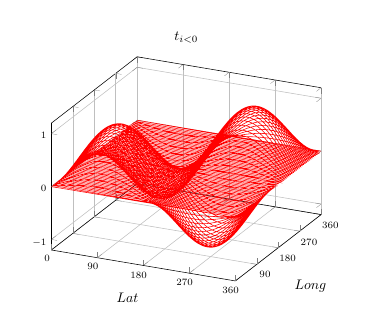
\begin{tikzpicture}[scale=0.50]
      \begin{axis} [
        title = {$t_{i<0}$},
        xtick = {0,90,...,360},
        ytick = {90,180,...,360},
        xlabel = $Lat$, ylabel = $Long$,
        ticklabel style = {font = \scriptsize},
	grid]
        \addplot3 [red, domain=0:360, samples=60] 
        	{ sin(x)*sin(y) };
        \end{axis}
        \end{tikzpicture}
        \centering{\footnotesize{Pre-treatment, no treatment response}}
    \end{column}
    % Split 2
    \begin{column}{0.33\linewidth}
      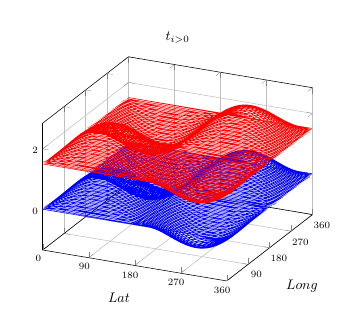
\begin{tikzpicture}[scale=0.50]
      \begin{axis} [
        title = {$t_{i>0}$},
        xtick = {0,90,...,360},
        ytick = {90,180,...,360},
        xlabel = $Lat$, ylabel = $Long$,
        ticklabel style = {font = \scriptsize},
	grid]
        \addplot3 [blue, domain=0:360, samples=60] 
        	{ sin(x)*sin(y) };
        \addplot3 [red, domain=0:360, samples=60] 
        	{ sin(x)*sin(y) + 1.5 };
        \end{axis}
        \end{tikzpicture}
        \centering{\footnotesize{Post-treatment, homogeneous response}}
    \end{column}
    % Split 3
    \begin{column}{0.33\linewidth}
      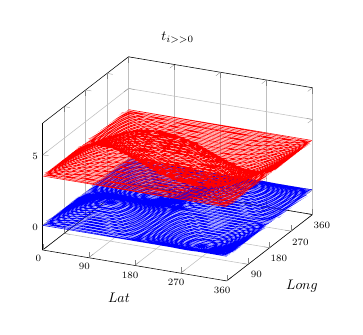
\begin{tikzpicture}[scale=0.50]
      \begin{axis} [
        title = {$t_{i>>0}$},
        xtick = {0,90,...,360},
        ytick = {90,180,...,360},
        xlabel = $Lat$, ylabel = $Long$,
        ticklabel style = {font = \scriptsize},
	grid]
        \addplot3 [blue, domain=0:360, samples=60] 
        	{ sin(x)*sin(y) };
        \addplot3 [red, domain=0:360, samples=60] 
        	{ sin(0.5*x)*3*sin(y) + 3.5 };
        \end{axis}
        \end{tikzpicture}
        \centering{\footnotesize{Post-treatment, heterogeneous response}}
    \end{column}
  \end{columns}

\end{frame}